\documentclass[12pt]{article}
\usepackage{paper,math}
\addbibresource{references.bib}

\title{Genomorientierte Bioinformatik - Report ExonSkipping}
\author{
  Malte Weyrich
}
\date{\today}

\hypersetup{
  pdftitle = {Example Paper Title},
  pdfauthor = {Author One, Author Two},
}

% Conditionally display thoughts (hide by switching to `\boolfalse`)
\boolfalse{INCLUDECOMMENTS}

\begin{document}

% Title Page -------------------------------------------------------------------
\maketitle
\begin{abstract}
	\textbf{Exon Skipping Splicing Events} (\textit{ES-SE}) beschreiben, wie co- oder posttranslational,
	manche Exons eines Transkripts durch das Splei\ss osom herausgeschnitten oder übersprungen werden, während
	in anderen Transkripten des selben Gens, diese weiterhin Teil der mRNA bleiben.
	Die \textit{ES-SE} lassen sich anhand von \textbf{Gene Transfer Format} (\textit{GTF}) files,
	also Genom Annotations Dateien ablesen und analysieren.
	Im Folgenden wird ein Programm zur Erkennung von allen \textit{ES-SE} innerhalb eines Genoms
	anhand seiner Logik, Laufzeit und Ergebnisse analysiert, wobei nur \textit{ES-SE} berücksichtigt werden,
	die protein-kodierende Transkripte betreffen. Das Programm wurde auf allen verfügbaren
	\textit{GTF} Dateien in \textit{/mnt/biosoft/praktikum/genprakt/gtfs/} ausgeführt.
    Der Source Code und alle dazugehörigen Komponenten sind auf \href{https://github.com/mweyrich28/exonSkipping}{GitHub} zu finden.
\end{abstract}

\newpage
\tableofcontents
\newpage


% Paper ------------------------------------------------------------------------

% ------------------------------------------------------------------------------
\section{ES-SE Definition}\label{sec:problem}
In einem Gen kann jedes Transkript jeweils mehrere \textit{ES-SE} haben.
Ein \textit{ES-SE} involviert immer jeweils mindestens eine \textbf{Splice Variant} (\textit{SV}) und einen
\textbf{Wild Type} (\textit{WT}). Beide dieser Begriffe beziehen sich auf Transkripte eines Gens $G$.
Ein \textit{SV} ist ein Transkript $T_{SV}$, welches ein Intron $I$ mit Startposition $I_{S}$ und Endposition
$I_{E}$ besitzt, was gleichzeitig bedeutet, dass es in $T_{SV}$ zwei Exons $A, B$ gibt, die $I$ flankieren. Somit endet $A$ bei $I_{S} - 1 = A_{E}$ und $B$ startet bei $I_{E} + 1 = B_{S}$.
Zudem ist die Position $B_{pos} - A_{pos} = 1$, wobei sich $A_{pos}$ auf die Position von Exon $A$ relativ gesehen
zu allen anderen Exons von $T_{SV}$ bezieht.
Ein \textit{WT} wäre nun ein weiteres Transkript $T_{WT}$ des selben Gens $G$, welches ebenfalls
zwei Exons $C, D$ besitzt mit $C_{pos} < D_{pos}$, wobei $C_{E} = I_{S} - 1$ und $D_{S} = I_{E} + 1$,
jedoch gilt für $C, D$: $D_{pos} - C_{pos} > 1$.
Dies bedeutet, dass die Exons von $T_{WT}$ zwischen $C$ und $D$ in $T_{SV}$ herausgesplei\ss t wurden.
Es kann pro Event mehrere \textit{SV}'s und \textit{WT}'s geben.

\section{Java Programm}
\subsection{Logik}\label{sec:logik}
Der Workflow der \textit{JAR} lässt sich in drei Schritte Aufteilen:
\begin{enumerate}
	\item[(A)] \textbf{Einlesen der \textit{GTF} Datei und Initialisierung der Datenstruktur}

		Zum einlesen wird die \textit{GTF} Datei zuerst nach relevanten Zeilen gefiltert, denn
		für uns sind momentan nur Zeilen relevant, die in der 3. Spalte entweder
		\textit{"exon"} oder \textit{"CDS"} stehen haben. Hierbei wird vermieden,
		die Methode \textit{String.split("\textbackslash t")} zu verwenden.
		Stattdessen wird in einem \textit{for loop} jedes Zeichen einzeln betrachtet.
		Dabei werden Zeilen die mit einem \textit{"\#"} anfangen direkt übersprungen.
		Für alle anderen Zeilen werden die Anzahl der \textit{tabs} gezählt und nach
		dem zweiten \textit{tab}, werden alle darauf folgenden Zeichen zu einem
		\textit{String} zusammen konkateniert, bis der dritte \textit{tab}
		erreicht wurde. Falls der entstandenen String $\in \left\{\text{"exon"}, \text{"CDS"} \right\}$, wird die
		Zeile einer \textit{ArrayList<String>} hinzugefügt, ansonsten wird mit der nächsten Zeile weiter gemacht.
		Diese Liste enthält am Ende alle relevanten Zeilen.
		Jede der relevanten Zeilen werden nun mit \textit{String.split("\textbackslash t")} in
		ein \textit{String[] mainComponents} geschrieben. Die \textit{attributeColumn} wird aus
		\textit{mainComponents} extrahiert (auch als ein \textit{String[]} Names \textit{attributes}),
		indem man \textit{mainComponents[mainComponents.length - 1]} am \textit{";"} splitted.

		Mit diesen zwei Komponenten pro Zeile wird als erstes die \textit{gene\_id} abgespeichert
		und überprüft, ob wir eine neue \textit{gene\_id} erreicht haben.
		Falls ja, wird ein neues Gen erstellt. Für die darauf folgenden Zeilen wird überprüft,
		ob wir ein neues Transkript erreicht haben. Neue Transkripte werden in einer
		\textit{ArrayList<Transkript>} des dazugehörigen Gens abgespeichert.
		Transkripte wiederum besitzen eine \textit{ArrayList<CodingDnaSequence> cdsList} und zwei
		\textit{HashMap<Integer, CodingDnaSequence>} \textit{cdsStartIndices}, \textit{cdsEndIndices}. Die Transkripte werden mit den dazugehörigen
		\textit{CodingDnaSequence}'s befüllt, wobei für jede erstellte \textit{CodingDnaSequence} die Start- und
		Endposition in den jeweiligen \textit{HashMap}'s als Key auf das erstellte Objekt verweisen.
		Zudem wird mit einer Zählvariable \textit{int cdsCount} die Position der \textit{CodingDnaSequence}'s
		innerhalb des Transkripts in dem \textit{CodingDnaSequence} Objekt gespeichert.

	\item[(B)] \textbf{Generieren der \textit{ES-SE}}

		Zum generieren der \textit{ES-SE} werden als erstes für alle in dem Genom abgespeicherten
		Gene, die dazugehörigen \textit{Introns} errechnet und in einem \textit{HashSet<Introns>}
		innerhalb des Gens abgespeichert. Dafür werden alle Transkripte eines Gens und deren
		\textit{CodingDnaSequence}'s angeschaut. Die Introns werden dann mit jeweils
		zwei \textit{CodingDnaSequence}'s berechnet
		(bei Genen die sich auf dem \textit{"-"} Strang befinden, müssen zuerst die
		\textit{cdsList}'s aller Transkripte invertiert werden und die
		Positionen der \textit{CodingDnaSequence}'s neu berechnet werden.
		Das ist später relevant für die Identifikation der \textit{WT}'s):
		\begin{verbatim}

// invert cdsList of transcripts
public void invertTranscripts() {
    for (int i = 0; i < transcripts.size(); i++) {
        Transcript currTranscript = transcripts.get(i);
        currTranscript.reversCdsList();
        // updating pos attribute of each cds
        for (int j = 0; j < currTranscript.getCdsList().size(); j++) {
            currTranscript.getCdsList().get(j).setPos(j);
        }
    }
}

// generating introns
for (Transcript transcript : transcripts) {
    for (int i = 0; i < transcript.getCdsList().size() - 1; i++) {
        int intronStart = transcript.getCdsList().get(i).getEnd() + 1;
        int intronEnd = transcript.getCdsList().get(i + 1).getStart() - 1;
        Intron intron = new Intron(intronStart, intronEnd);
        introns.add(intron);
    }
}
    \end{verbatim}

		Anschlie\ss end wird für jedes Gen $G$ über die Intron Liste iteriert. Für jedes Intron $I$
		müssen alle Transkripte von $G$ nach \textit{CodingDnaSequence}'s $A, B$ durchsucht werden, die
		die Bedingung $A_{E} + 1 = I_{S}$ und $B_{S} - 1 = I_{E}$. Dies kann mit Hilfe der zwei
		\textit{HashMap<Integer, CodingDnaSequence>} Objekte durchgeführt werden.
		Zudem wir für jedes Intron $I$ jeweils 4 leere \textit{HashSet<String>}'s erstellt:
		\begin{enumerate}
			\item[1.] \textit{SV\_INTORN}: enthält \textit{"intronStart:intronEnd"} des momentanen Introns $I$
			\item[2.] \textit{SV\_PROTS}: enthält die \textit{proteinId} von \textit{CodingDnaSequence} $A$
			\item[3.] \textit{WT\_INTORN}: enthält alle \textit{"intronStart:intronEnd"} Koordinaten, die zwischen $A$ und $B$ liegen
			\item[4.] \textit{WT\_PROTS}: enthält die \textit{proteinId}'s von allen \textit{CodingDnaSequence}'s die zwischen $A$ und $B$ liegen
		\end{enumerate}
		Nun gibt es zwei Möglichkeiten:
		\begin{enumerate}
			\item  $A_{E} + 1 = I_{S}$ und $B_{S} - 1 = I_{E}$ und $B_{pos} - A_{pos} = 1$
			\item  $A_{E} + 1 = I_{S}$ und $B_{S} - 1 = I_{E}$ und $B_{pos} - A_{pos} > 1$
		\end{enumerate}

		Falls $i$ eintrifft, handelt es sich um ein \textit{SV} und es wird die \textit{proteinId} von \textit{CodingDnaSequence} $A$
		in \textit{SV\_PROTS} aufgenommen.
		Ansonsten werden bei Fall $ii$ alle \textit{proteinId}'s der \textit{CodingDnaSequence}'s zwischen $A$ und $B$ zu
		\textit{WT\_PROTS} und alle Introns zwischen $A$ und $B$ zu \textit{WT\_INTORN} hinzugefügt.
		Dabei werden ebenfalls Werte wie \textit{min/max\_skipped\_exon/bases} berechnet:
		\begin{verbatim}
// add all introns of WT to WT_INTRON and all cdsids/prot_ids to WT_prots
int skippedBases = 0;
for (int i = cdsFront.getPos() ; i < cdsBehind.getPos(); i++) {
    int wtIntronStart = cdsList.get(i).getEnd() + 1;
    int wtIntronEnd = cdsList.get(i+1).getStart();
    WT_INTRON.add(wtIntronStart + ":" + wtIntronEnd);

    // like this i add many ids twice but that's fine :)
    WT_PROTS.add(cdsFront.getId());
    WT_PROTS.add(cdsBehind.getId());

    if (i > cdsFront.getPos() && i < cdsBehind.getPos()) {
        // we are in a cds that was skipped
        // → get end - start + 1 = length → add to skipped bases
        skippedBases += cdsList.get(i).getEnd() 
                        - cdsList.get(i).getStart() + 1;
    }
}
    \end{verbatim}
		Ein \textit{ES-SE} wird nur in die \textit{ArrayList<String> events} aufgenommen, falls es für das momentane
		Intron $I$ mindestens einen \textit{WT} gab.

	\item[(C)] \textbf{Erstellen der \textit{<out>.tsv} Datei}

		Die \textit{ArrayList<String> events} enthält nun alle \textit{ES-SE} als \textit{String} in bereits
		korrekter Formatierung. In einem \textit{for loop} wird die Lösung Zeile für Zeile in ein \textit{out.tsv}
		geschrieben.
\end{enumerate}

\subsection{Korrektheit}
In der Einleseroutine werden alle relevanten Zeilen verarbeitet und das Genom
korrekt Initialisiert, sofern die Struktur von dem \textit{GTF} den \href{https://asia.ensembl.org/info/website/upload/gff.html}{offiziellen Konventionen} folgt und die jeweiligen
\textit{CodingDnaSequence}'s in korrekter Reihenfolge (je nach \textit{"-"/"+"} Strang) vorliegen.
Zudem werden, falls es keine \textit{"protein\_id"} für eine gegebene Zeile gibt, nach der
\textit{"ccdsid"} gesucht und falls es diese nicht gibt, wird die \textit{"protein\_id"}
mit \textit{"NaN"} überschrieben. So werden alle Zeilen, die \textit{"CDS"} in ihrer
dritten Spalte stehen haben, genutzt, um das Genom aufzufüllen.
Für das Errechnen der \textit{ES-SE} in Schritt (B) gilt folgendes:
Alle möglichen Introns in einem Gen werden überprüft und für jedes Intron
werden alle Transkripte des jeweiligen Gens auf bei $I_{S} - 1$ endende  und
bei $I_{E} + 1$ startende \textit{CodingDnaSequence}'s $A, B$ abgefragt. Für
jeden \textit{SV} oder \textit{WT} Kandidaten wird anschlie\ss end geschaut,
ob es zwischen $A$ und $B$ weitere \textit{CodingDnaSequence}'s gibt und
je nach dem ein \textit{ES-SE} entdeckt oder nicht.
So ist das Programm unter der Annahme, dass die \textit{GTF} Datei fehlerfrei ist, korrekt.



\subsection{Laufzeit}
Die Laufzeitanalyse wird in die drei Segmente aus \ref{sec:logik} unterteilt.
\begin{enumerate}
	\item[(A)] \textbf{Einlesen der \textit{GTF} Datei und Initialisierung der Datenstruktur}

		Für eine \textit{GTF} Datei mit $m$ Zeilen benötigt die Selektion der relevanten Zeilen
		schon mal mindestens $m$ Vergleiche, da jede Zeile überprüft werden muss.
		Für jede Zeile wird ein Substring ab dem zweiten \textit{Tab} bis zum dritten \textit{Tab} erstellt (au\ss er bei Kommentaren, diese werden übersprungen).
		Die Anzahl der Vergleiche pro Zeile ist kleiner als die Länge der Zeile (da wir ab dem dritten \textit{Tab} abbrechen) und lässt
		sich als $a < m.length$ beschreiben. Also
		\begin{equation}
			\mathcal{O}(m \cdot a) \implies \mathcal{O}(m)
		\end{equation}
		,da $a$ eine Konstante ist.

		Bei einer \textit{GTF} Datei mit $m$ validen Zeilen (d.h. jede Zeile hat entweder einen \textit{"exon"} oder \textit{"CDS"} Eintrag) bleiben
		nach dem Filtern $m$ Zeilen übrig.
		Für jede dieser Zeilen muss:
		\begin{enumerate}
			%% https://softwareengineering.stackexchange.com/questions/331909/whats-the-complexity-of-javas-string-split-function
			\item Die Zeile am \textit{Tab} geteilt werden:
			      \begin{equation}
				      \mathcal{O}(n)
			      \end{equation}
			      , wobei $n$ die Länge der Zeile ist.
			\item Die letzte Komponente aus i. am \textit{;} geteilt werden: lässt sich ebenfalls mit
			      \begin{equation}
				      \mathcal{O}(n)
			      \end{equation}
			      von oben beschränken.
			\item Die \textit{gene\_id} aus den Attributen aus ii. mit \textit{String parseAttributes(String[] attributeEntries, String attributeName)}
			      abfragen, also:
			      \begin{equation}
				      \mathcal{O}(e \cdot e_{l})
			      \end{equation}
			      , wobei $e$ die Länge des \textit{attributeEntries} Arrays ist und
			      $e_{l}$ die Länge des längsten Eintrags in \textit{attributeEntries} ist, da wir im Worst Case
			      über alle Einträge in \textit{attributeEntries} iterieren ($e$) und für jeweils jeden Eintrag
			      mindesten vier String Operationen (\textit{trim()}, \textit{indexOf()}, zwei mal \textit{substring()})
			      und eine Vergleichsoperation (\textit{equals()}) aufrufen, welche maximal $e_{l}$ viele
			      Operationen benötigen. Also $\mathcal{O}(e \cdot 5 \cdot e_{l}) = \mathcal{O}(e \cdot e_{l})$.
			      Für jedes weitere Vorkommen von \textit{parseAttributes()} wird diese Komplexität angenommen.
			\item Ein neues Gen initialisiert werden und der \textit{gene\_name} abgefragt werden (falls ein neues Gen erreicht wurde), also:
			      \begin{equation}
				      \mathcal{O}(1 + e \cdot e_{l})
			      \end{equation}
			\item Die \textit{transcript\_id} abgefragt werden, also
			      \begin{equation}
				      \mathcal{O}(e \cdot e_{l})
			      \end{equation}
			\item Falls es sich um einen \textit{"CDS"} Eintrag handelt, muss die \textit{protein\_id} abgefragt werden, also:
			      \begin{equation}
				      \mathcal{O}(e \cdot e_{l})
			      \end{equation}
			      und in Konstanter Zeit ggf. neue Objekte erstellt, oder auf bereits existierende Objekte
			      zugreifen, um ein neues \textit{CodingDnaSequence} Objekt zu erstellen.
		\end{enumerate}

		Insgesamt hat die Einleseroutine also eine Komplexität von
		\[
			(A) \hspace{1em} \mathcal{O}(m \cdot 2 \cdot n \cdot 4 \cdot  (e \cdot e_{l})) = \mathcal{O}(m \cdot n \cdot e \cdot e_{l}) \in  \mathcal{O}(m^{2})
			.\]
		,da $m > n > e_{l} >= e$ und somit $\mathcal{O}(m^{2})$ eine valide obere Schranke darstellt.
	\item[(B)] \textbf{Generieren der \textit{ES-SE}}

		Sei $g$ die Anzahl an Genen in unserem Genom. Da wir vom Worst Case ausgehen sagen wir,
		dass sich jedes Gen auf dem \textit{"-"} Strang befindet.
		So muss zuerst in jedem Transkript jedes Gens die \textit{cdsList} invertiert werden.
		Dies geschieht in:
		\begin{equation}
			\mathcal{O}(g \cdot g_{t} \cdot 2 \cdot t_{c}) = \mathcal{O}(g \cdot g_{t} \cdot t_{c})
		\end{equation}
		, wobei $g_{t}$ die grö\ss te Anzahl an Transkripten von $g$ ist und $t_{c}$ die längste \textit{cdsList} eines Transkripts ist.
		Die Konstante $2$ kommt zustande, da zuerst die \textit{cdsList} mit \textit{Collections.reverse()} umgekehrt wird ($\mathcal{O}(g_{t})$) und
		dann nochmals in $\mathcal{O}(g_{t})$ durchlaufen wird, um die in den \textit{CodingDnaSequence} Objekten gespeicherte Position
		anzupassen.
		Dann werden für jedes Gen $g$ die Introns generiert. Dies geschieht ebenfalls in
		\begin{equation}
			\mathcal{O}(g \cdot g_{t} \cdot t_{c})
		\end{equation}
		Die \textit{ES-SE} werden in der \textit{getEvents()} Methode berechnet.
		Dafür müssen für alle Gene alle Introns und alle Transkripte überprüft werden.
		Also schon mal $\mathcal{O}(g \cdot g_{i} \cdot g_{t})$.
		Hier ist $g_{i}$ die grö\ss te Anzahl an Introns von allen Genen und $g_{t}$ wieder
		die grö\ss te Anzahl an Transkripten aller Gene. Alle anderen Operationen sind
		konstant in ihrer Komplexität, da bei ihnen lediglich bereits existente Werte
		in \textit{HashMaps} oder Objekten abgefragt werden.
		Nur falls ein \textit{WT} entdeckt wird, wird in einem \textit{for loop} über die
		\textit{CodingDnaSequence}'s zwischen $C$ und $D$ (siehe \ref{sec:problem}. ES-SE Definition) iteriert.
		Sei $mSE$ (= maxSkippedExons) also die von allen \textit{ES-SE} eines Genoms
		maximale Anzahl an übersprungenen Exons, so wäre die gesamte Komplexität von
		II:
		\begin{equation}
			(B) \hspace{1em} \mathcal{O}(2 \cdot (g \cdot g_{t} \cdot t_{c}) + g \cdot g_{i} \cdot g_{t} \cdot mSE) = \mathcal{O}(\overbrace{g \cdot g_{t} \cdot t_{c}}^{\shortstack{\scriptsize\text{invertTranscripts()} \\ \text{\scriptsize\& generateIntrons()}}} + \underbrace{g \cdot g_{i} \cdot g_{t} \cdot mSE}_{\text{getEvents()}} )
		\end{equation}

	\item[(C)] \textbf{Erstellen der \textit{<out>.tsv} Datei}

		Hat eine Komplexität von
		\begin{equation}
			(C) \hspace{1em} \mathcal{O}(E)
		\end{equation}
		, wenn $E$ die Menge aller \textit{ES-SE} ist.
\end{enumerate}

Zusammenfassend also eine Gesamtkomplexität von:
\begin{equation}
	(A) + (B) + (C) = \mathcal{O}( m^{2} + g \cdot g_{t} \cdot t_{c} + g \cdot g_{i} \cdot g_{t} \cdot mSE + E) \in \mathcal{O}(m^{2})
\end{equation}
, da $m^{2} > g \cdot g_{t} \cdot t_{c}$ und $m^{2} > g \cdot g_{i} \cdot g_{t} \cdot mSE + E$.
Das bedeutet, dass die Kosten der Gesamtoperation im Wesentlichen durch das Einlesen und Strukturieren der Daten (Teil A) dominiert werden,
wenn man davon ausgeht, dass $m$ in der Praxis größer als $g$, $g_{t}$, $t_{c}$, $g_{i}$ und $mSE$ ist.

\subsection{Benchmarking}
Für das Benchmarking wird jeweils \textit{/mnt/biosoft/praktikum/genprakt/gtfs/Homo\_sapiens.GRCh38.86.gtf} verwendet, da sie die grö\ss te \textit{GTF} Datei mit $1.4GB$ ist.

\begin{figure}[htpb]
	\centering
	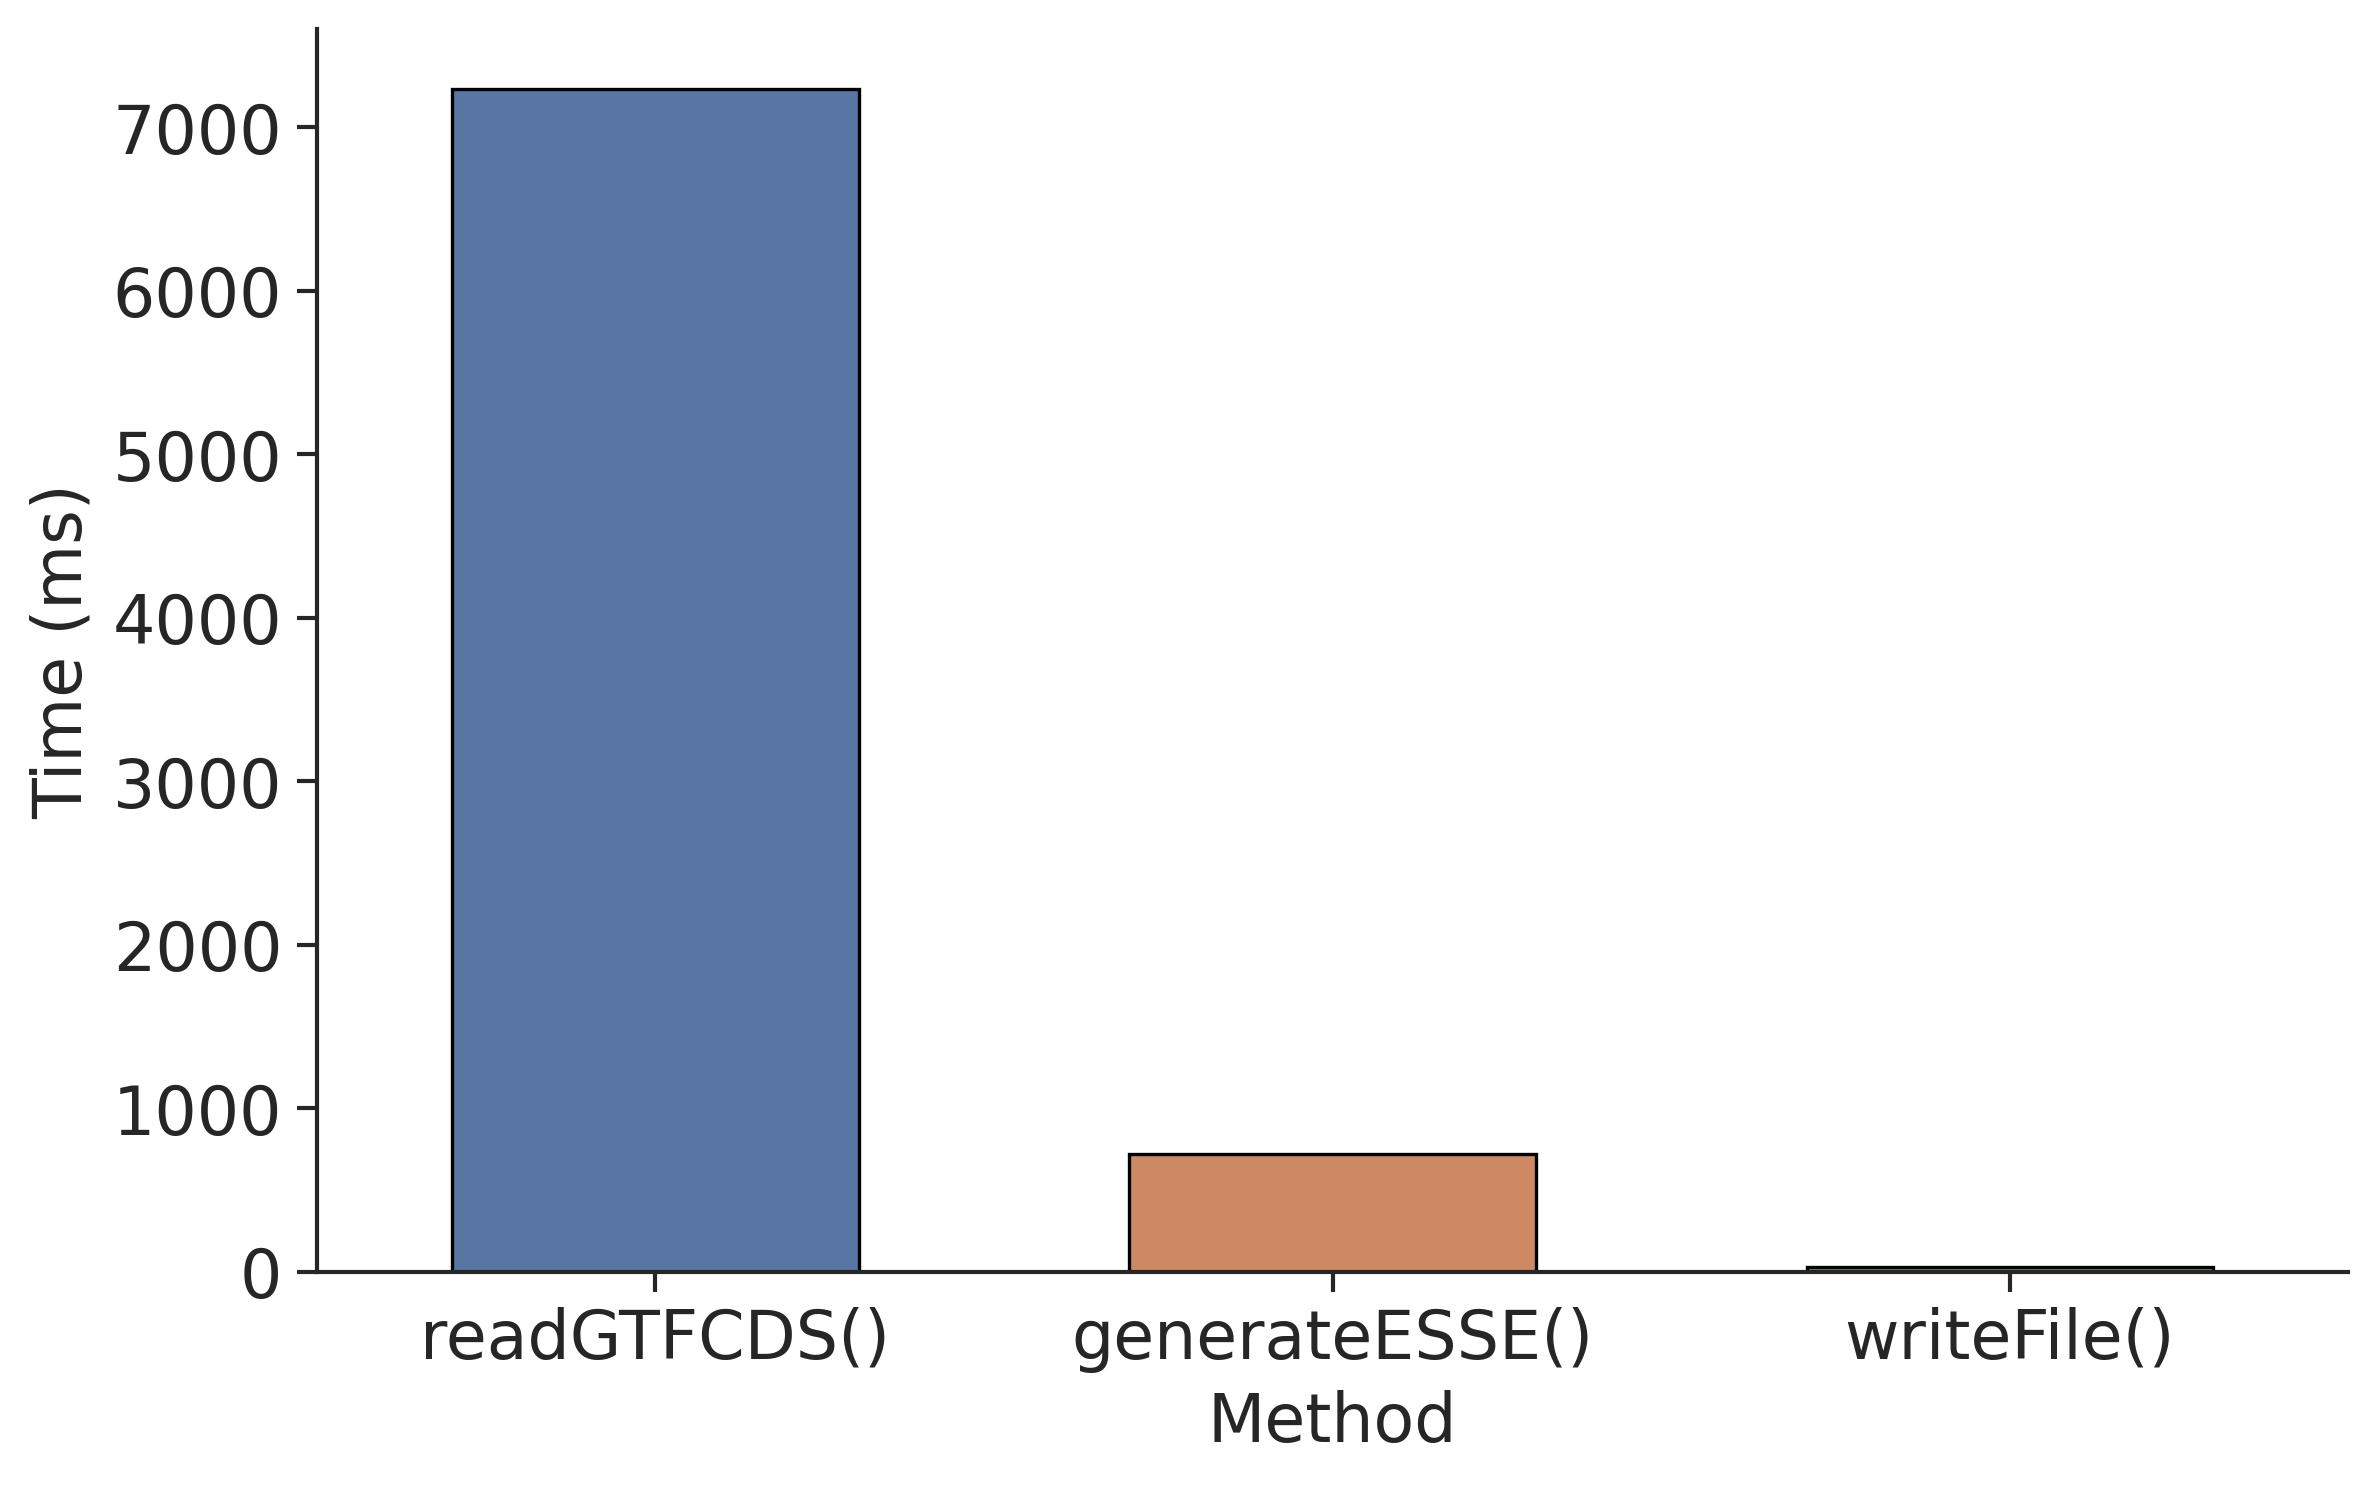
\includegraphics[width=0.8\textwidth]{./plots/benchmark_time.jpg}
	\caption{Methoden Durchschnittslaufzeit der Schritte A, B, C  in ms nach 30 facher Ausführung auf Hardware: \textit{AMD Ryzen 7 PRO 4750U with Radeon Graphics (16) @ 1.700GHz}}

	\label{fig:-plots-benchmark_time-jpg}
\end{figure}

In \ref{fig:-plots-benchmark_time-jpg} ist eindeutig zu sehen, wie das Einlesen und Initialisieren
der Datenstruktur aus Schritt (A), die Dominante Komponente mit $6721ms$ bildet, während die Generierung der
\textit{ES-SE} lediglich $262ms$ benötigt.
Für die Memory Allocations wurde der in \textit{IntelliJ} zur Verfügung gestellter \textit{Profiler} verwendet.
Der Schritt (A) ist auch hier dominant und beansprucht insgesamt $10.33GB$ an Speicher.
Von diesen $10.33GB$ werden alleine $6.72GB$ ($65.18\%$) für die Methode \textit{String.split()} benötigt.
Für die Berechnung der \textit{ES-SE} werden lediglich $288.11MB$ in Anspruch genommen.
% TODO: Kurze Diskussion maybe <30.10.24, Malte Weyrich> %



\section{Ergebnisse}
Für die Analyse wurde die \textit{GTF} Datei \textit{/mnt/biosoft/praktikum/genprakt/gtfs/Saccharomyces\_cerevisiae.R64-1-1.75.gtf} ausgelassen,
da es hier zu keinen \textit{ES-SE} gekommen ist. Die Ursache dafür ist wahrscheinlich, dass
es, obwohl es in der Hefe auch zu Splicing kommt, in der gegebenen \textit{GTF} Datei keine protein-kodierenden Transkripte mit
Splicing gab, oder allgemein keine \textit{ES-SE} aufgetreten sind. Zusätzlich werden die \textit{GTF} Dateien und die
dazugehörigen Ergebnisse mit den folgenden IDs bezeichnet:

\begin{table}[htpb]
	\centering
	\caption{Liste der verwendeten \textit{GTF} Dateien}
	\label{tab:label}
	\begin{tabular}{l|c}
		\textbf{ID} & \textbf{\textit{GTF} Datei} \\ \hline
		h.ens.67    & Homo\_sapiens.GRCh37.67.gtf \\
		h.ens.75    & Homo\_sapiens.GRCh37.75.gtf \\
		h.ens.86    & Homo\_sapiens.GRCh38.86.gtf \\
		h.ens.90    & Homo\_sapiens.GRCh38.90.gtf \\
		h.ens.93    & Homo\_sapiens.GRCh38.93.gtf \\
		m.ens.75    & Mus\_musculus.GRCm38.75.gtf \\
		h.gc.10     & gencode.v10.annotation.gtf  \\
		h.gc.25     & gencode.v25.annotation.gtf  \\
	\end{tabular}
\end{table}


Als erstes wird die Anzahl an aller protein-kodierenden Gene einer \textit{GTF} mit der Anzahl an Genen mit \textit{ES-SE} und der Gesamtanzahl an \textit{ES-SE}
verglichen:

\begin{figure}[htpb]
	\centering
	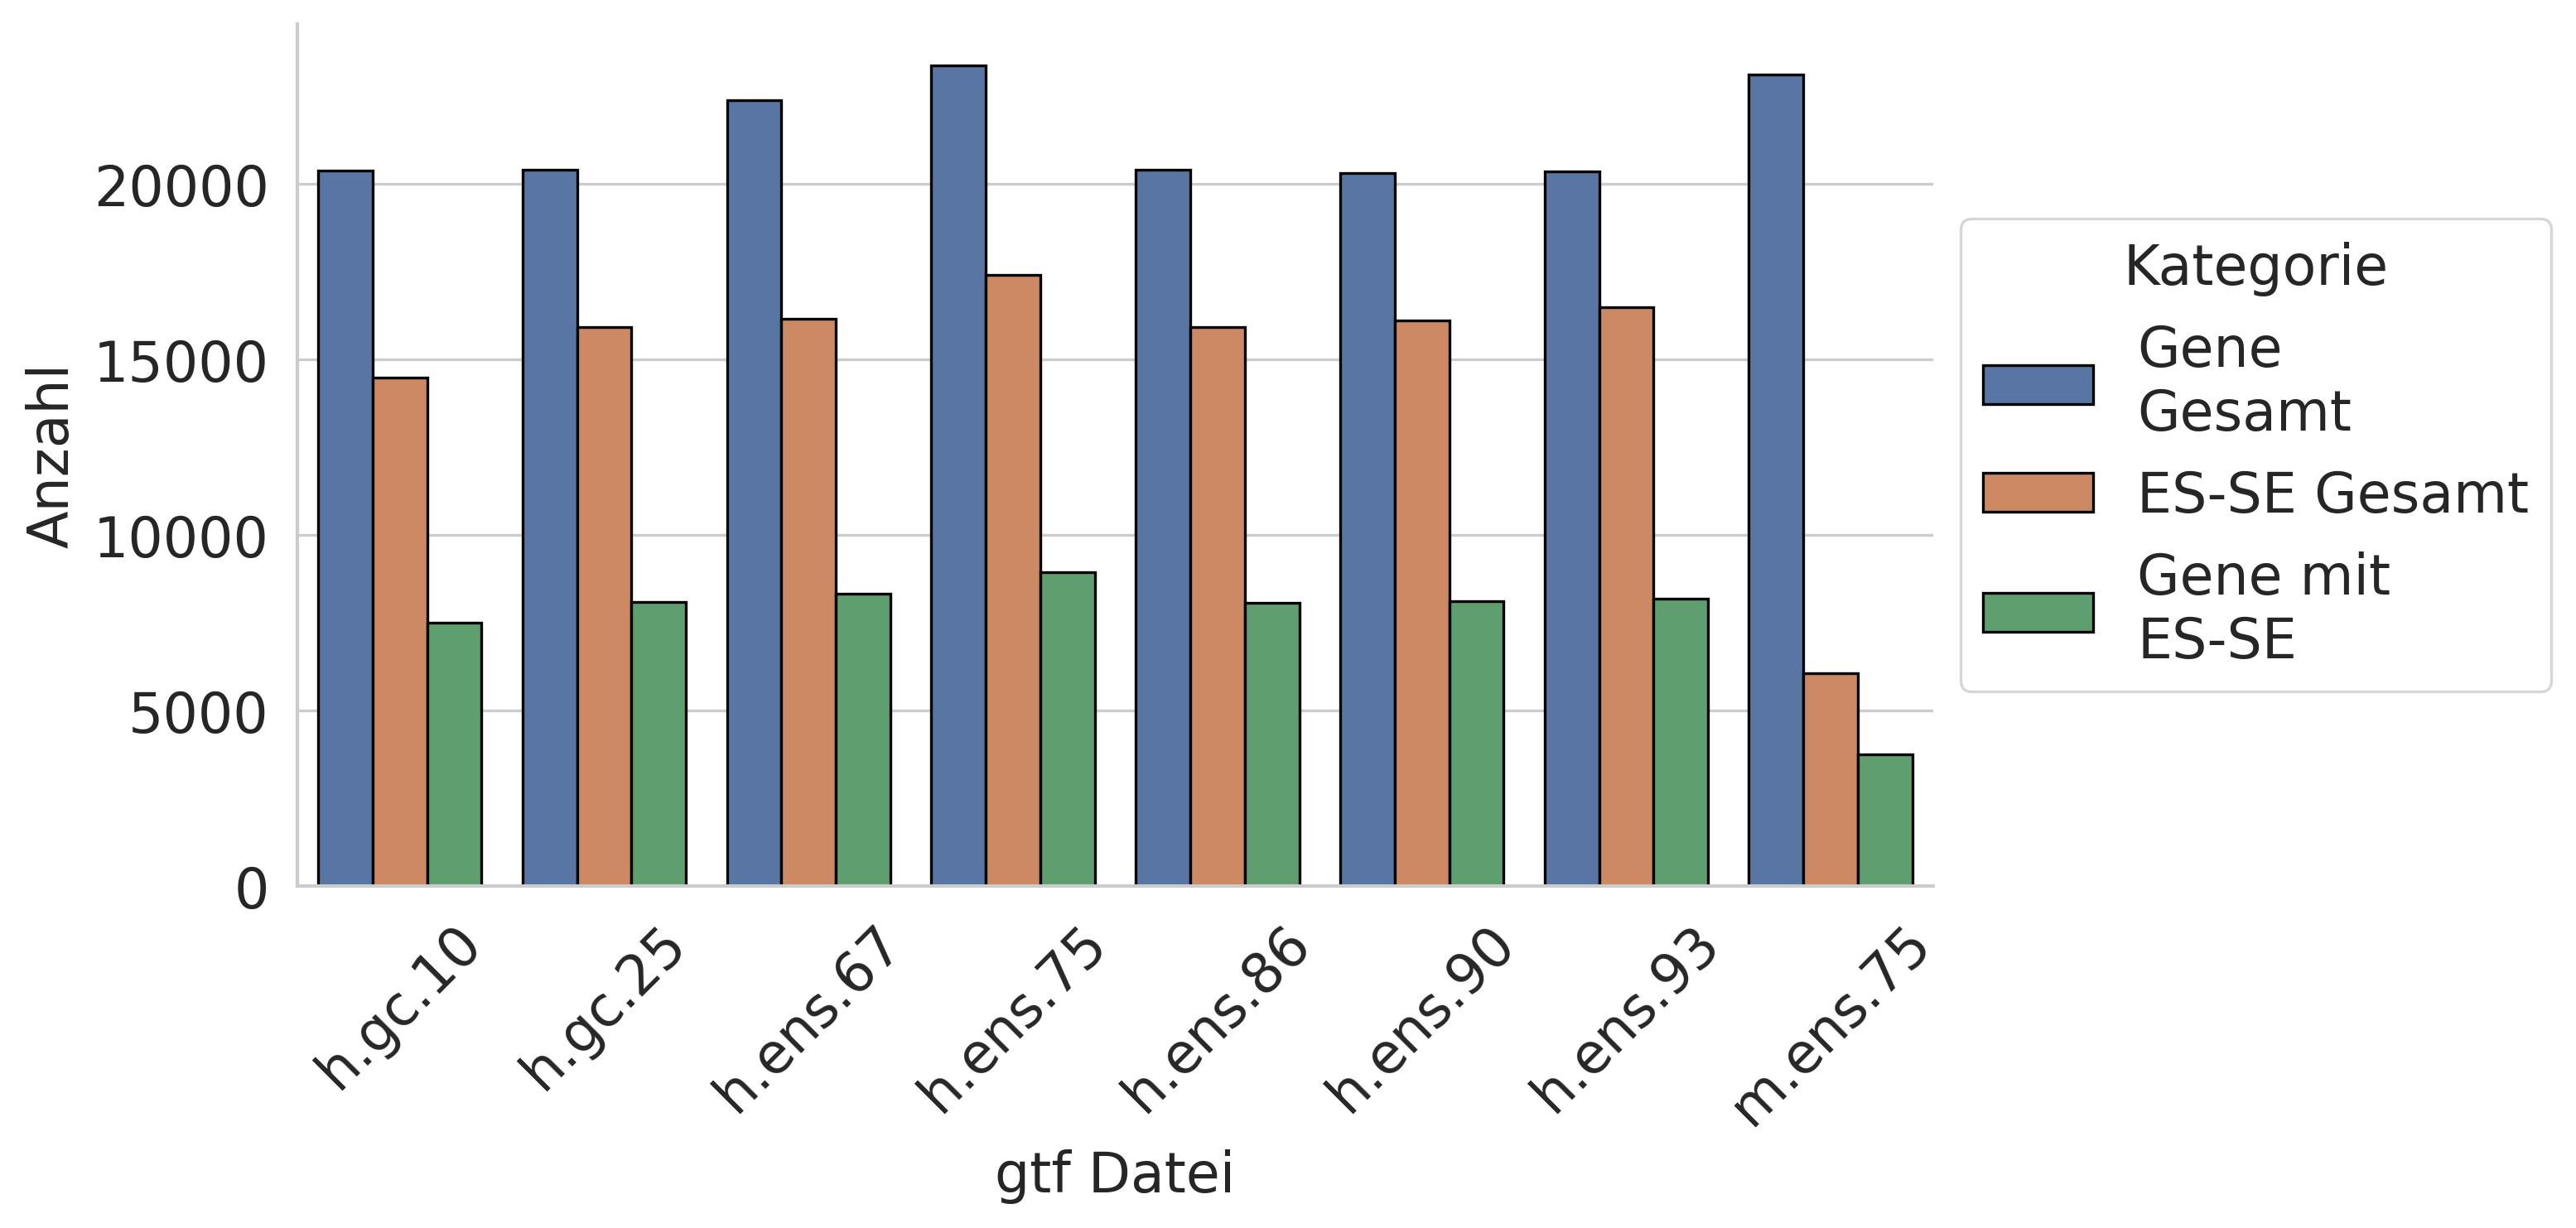
\includegraphics[width=0.8\textwidth]{./plots/genes.jpg}
	\caption{Vergleich zwischen Gene Gesamt, Gene mit \textit{ES-SE} und \textit{ES-SE} Gesamt pro \textit{GTF}}
	\label{fig:-plots-genes-jpg}
\end{figure}

In Abbildung \ref{fig:-plots-genes-jpg} sieht man, wie die Anzahl an Genen in den verschiedenen \textit{GTF} Dateien des
Menschen in einem Intervall von $[20320; 23393]$ variieren. Dies liegt daran, dass die
\textit{GTF} Dateien jeweils von unterschiedlichen Assemblies und Annotations Versionen stammen,
welche beide einen starken Einfluss auf die resultierende \textit{GTF} haben (und somit auch auf das Ergebnis der \textit{JAR}).
Wie zu erwarten, hat bei den zum Menschen zugehörigen \textit{GTF} Dateien, die mit den meisten Genen auch die meisten \textit{ES-SE}.
Die Dateien \textit{"h.gc.25"}, \textit{"h.ens.67"}, \textit{"h.ens.86"}, \textit{"h.ens.90"}, \textit{"h.ens.93"} haben alle eine sehr
ähnliche Verteilung der \textit{"ES-SE Gesamt"} und \textit{"Gene mit ES-SE"} Kategorie, obwohl die \textit{GTF} Datei von
\textit{"h.ens.67"} mehr Gene beinhaltet, als die drei anderen \textit{GTF} Dateien.
\textit{"h.gc.10"} scheint am wenigsten \textit{Gene mit ES-SE} und \textit{"ES-SE Gesamt"} zu besitzen.
Bei der Maus wiederum gibt es vergleichsweise wenige \textit{ES-SE}, obwohl es insgesamt fast genau so viele
protein-kodierende Gene gibt (23119) wie in \textit{"h.ens.75"} (23393).

Unter Einbezug der Abbildungen \ref{fig:-plots-skipped_bases-jpg} und \ref{fig:-plots-skipped_exons-jpg}, sind die
selben vier Trends zu beobachten, die sich in Abbildung \ref{fig:-plots-genes-jpg} bereits andeuten:

\begin{figure}[htpb]
	\centering
	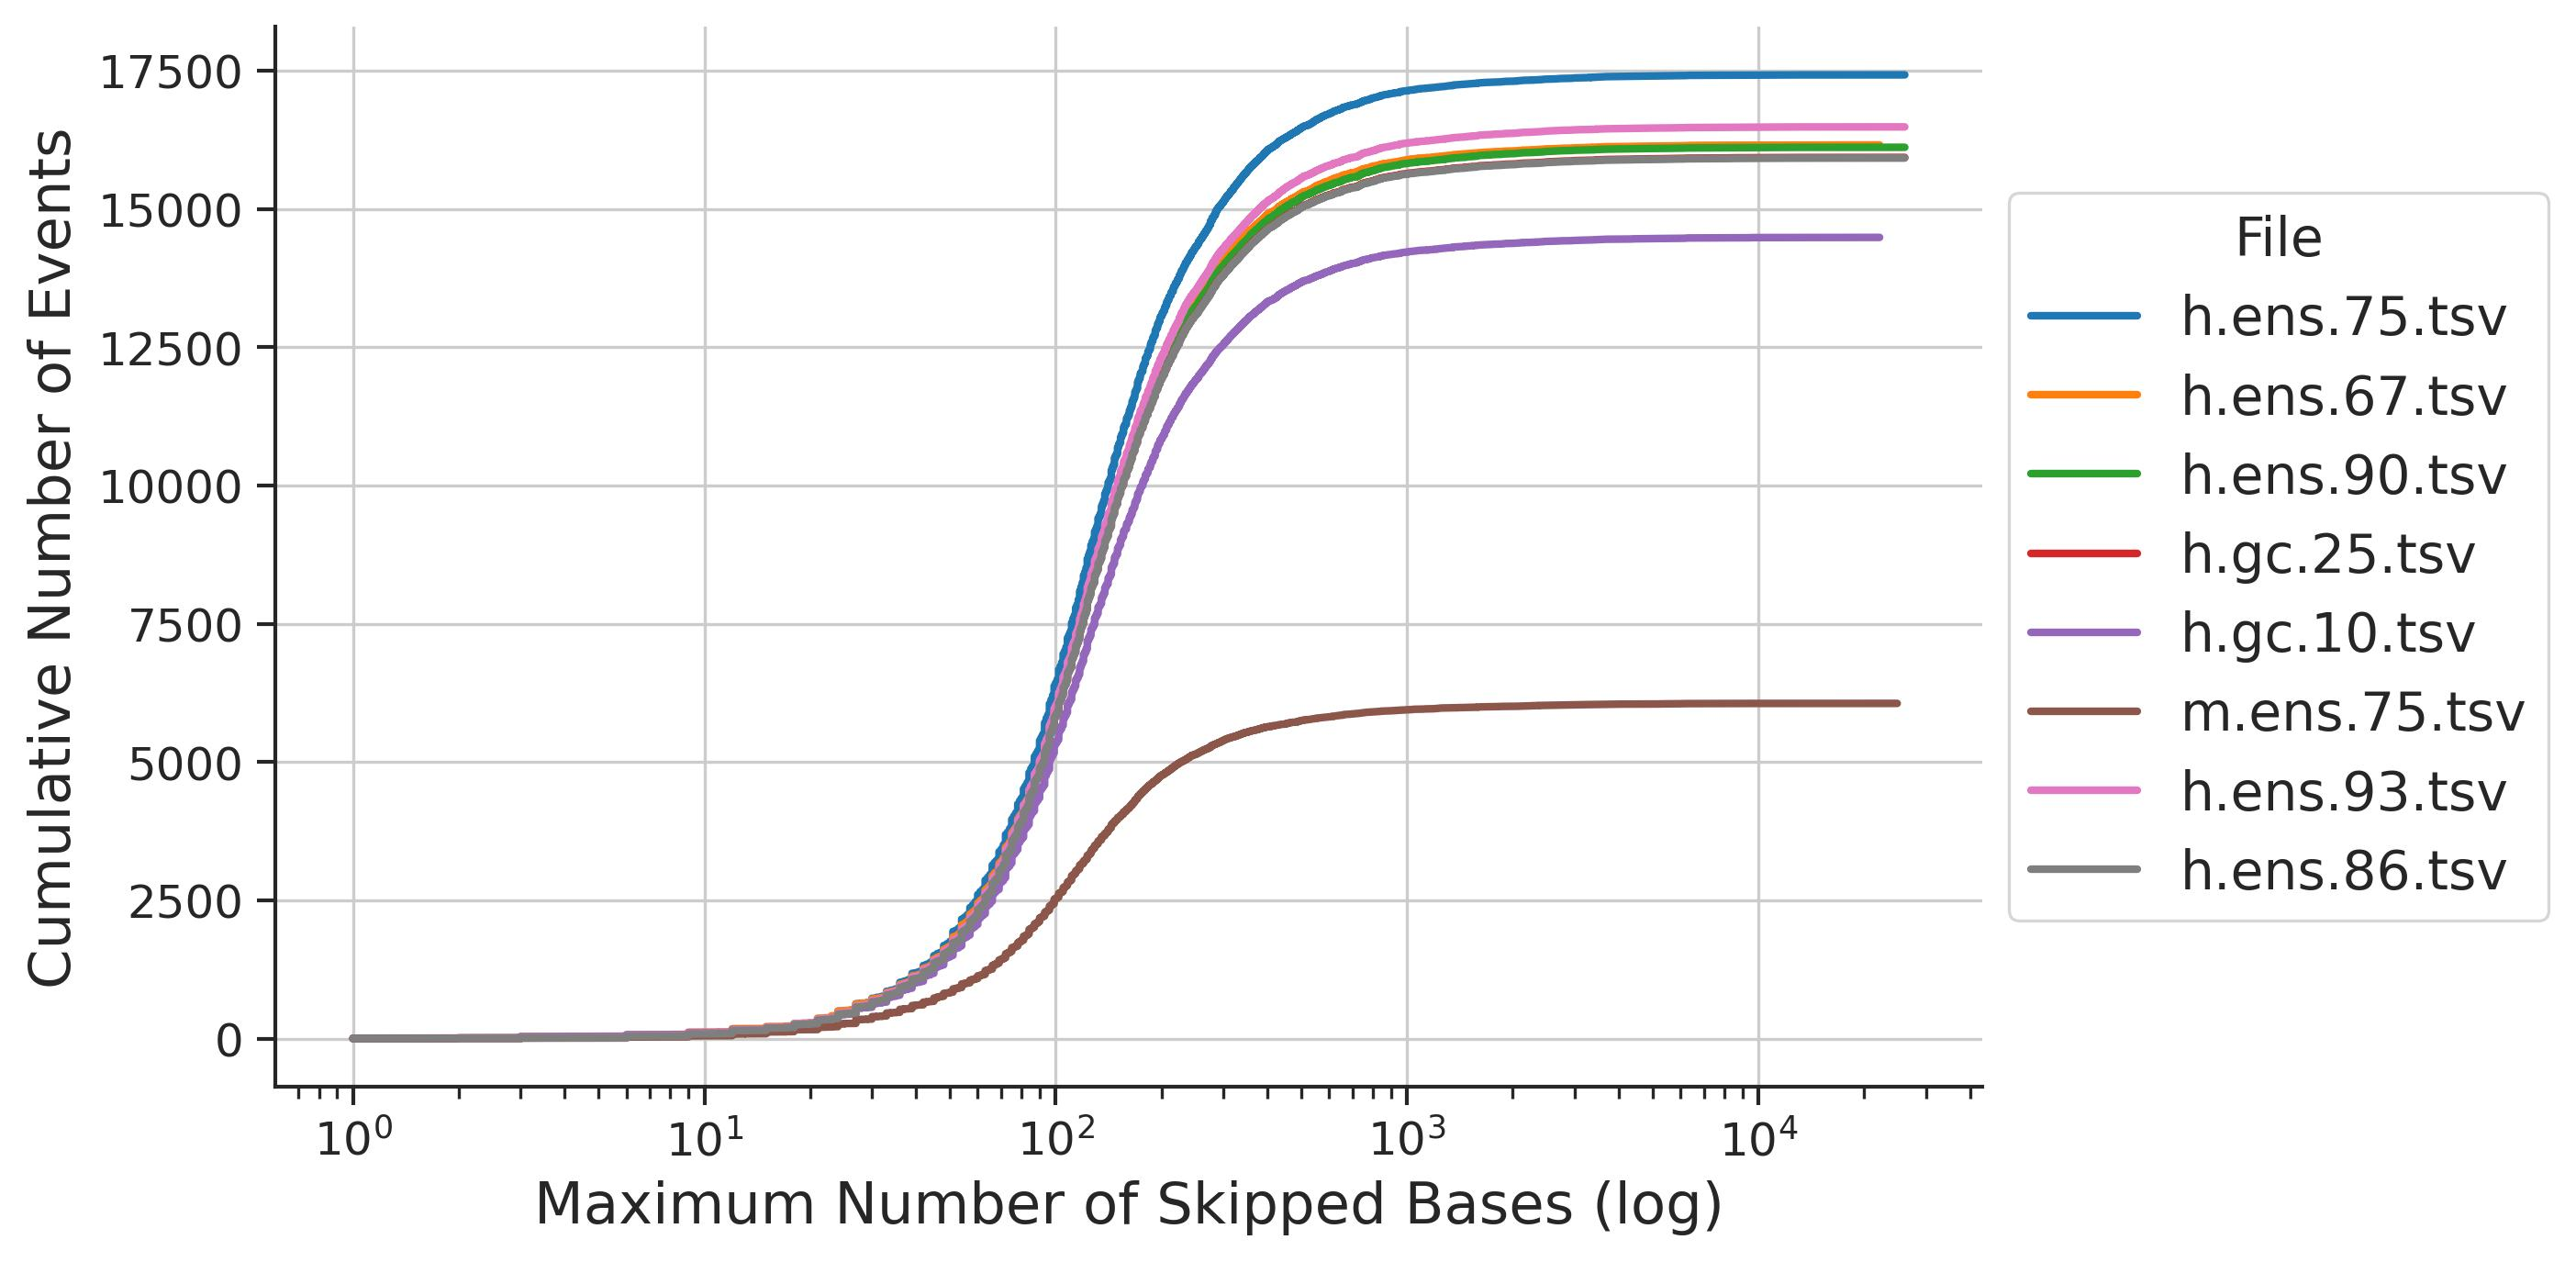
\includegraphics[width=0.8\textwidth]{./plots/skipped_bases.jpg}
	\caption{Kumulative Verteilung der übersprungenen Basen pro \textit{GTF}}
	\label{fig:-plots-skipped_bases-jpg}
\end{figure}


Abbildung \ref{fig:-plots-skipped_bases-jpg} zeigt die kumulative Verteilung der übersprungenen Basen pro \textit{GTF}.
Alle Kurven zeigen einen charakteristischen S-förmigen Verlauf, was auf ein ähnliches grundlegendes Muster im \textit{ES-SE} Verhalten
hindeutet. Es bilden sich hauptsächlich zwei Plateaus aus:
Ein höheres Plateau bei etwa 15.000-17.500 übersprungenen Basen für die vom Mensch stammenden \textit{GTF} Dateien
und ein niedrigeres Plateau bei etwa 6.000 übersprungenen Basen für die Maus.
Die zwei Ausrei\ss er (\textit{"h.ens.75"} und \textit{"h.gc.10"}) des höheren Plateaus sind wieder auf die jeweils
grö\ss te und kleinste Anzahl an Genen mit \textit{ES-SE} innerhalb der Humanen \textit{GTF} Dateien zurückzuführen.

Der steilste Anstieg der Kurven erfolgt im Bereich zwischen 100 und 1.000 übersprungenen Basen, was darauf hindeutet,
dass die meisten \textit{ES-SE} in diesem Größenbereich stattfinden.
Die logarithmische Skalierung der x-Achse verdeutlicht, dass die \textit{ES-SE} über mehrere Größenordnungen hinweg auftreten,
von einzelnen Basen bis hin zu mehreren tausend Basen.

\begin{figure}[htpb]
	\centering
	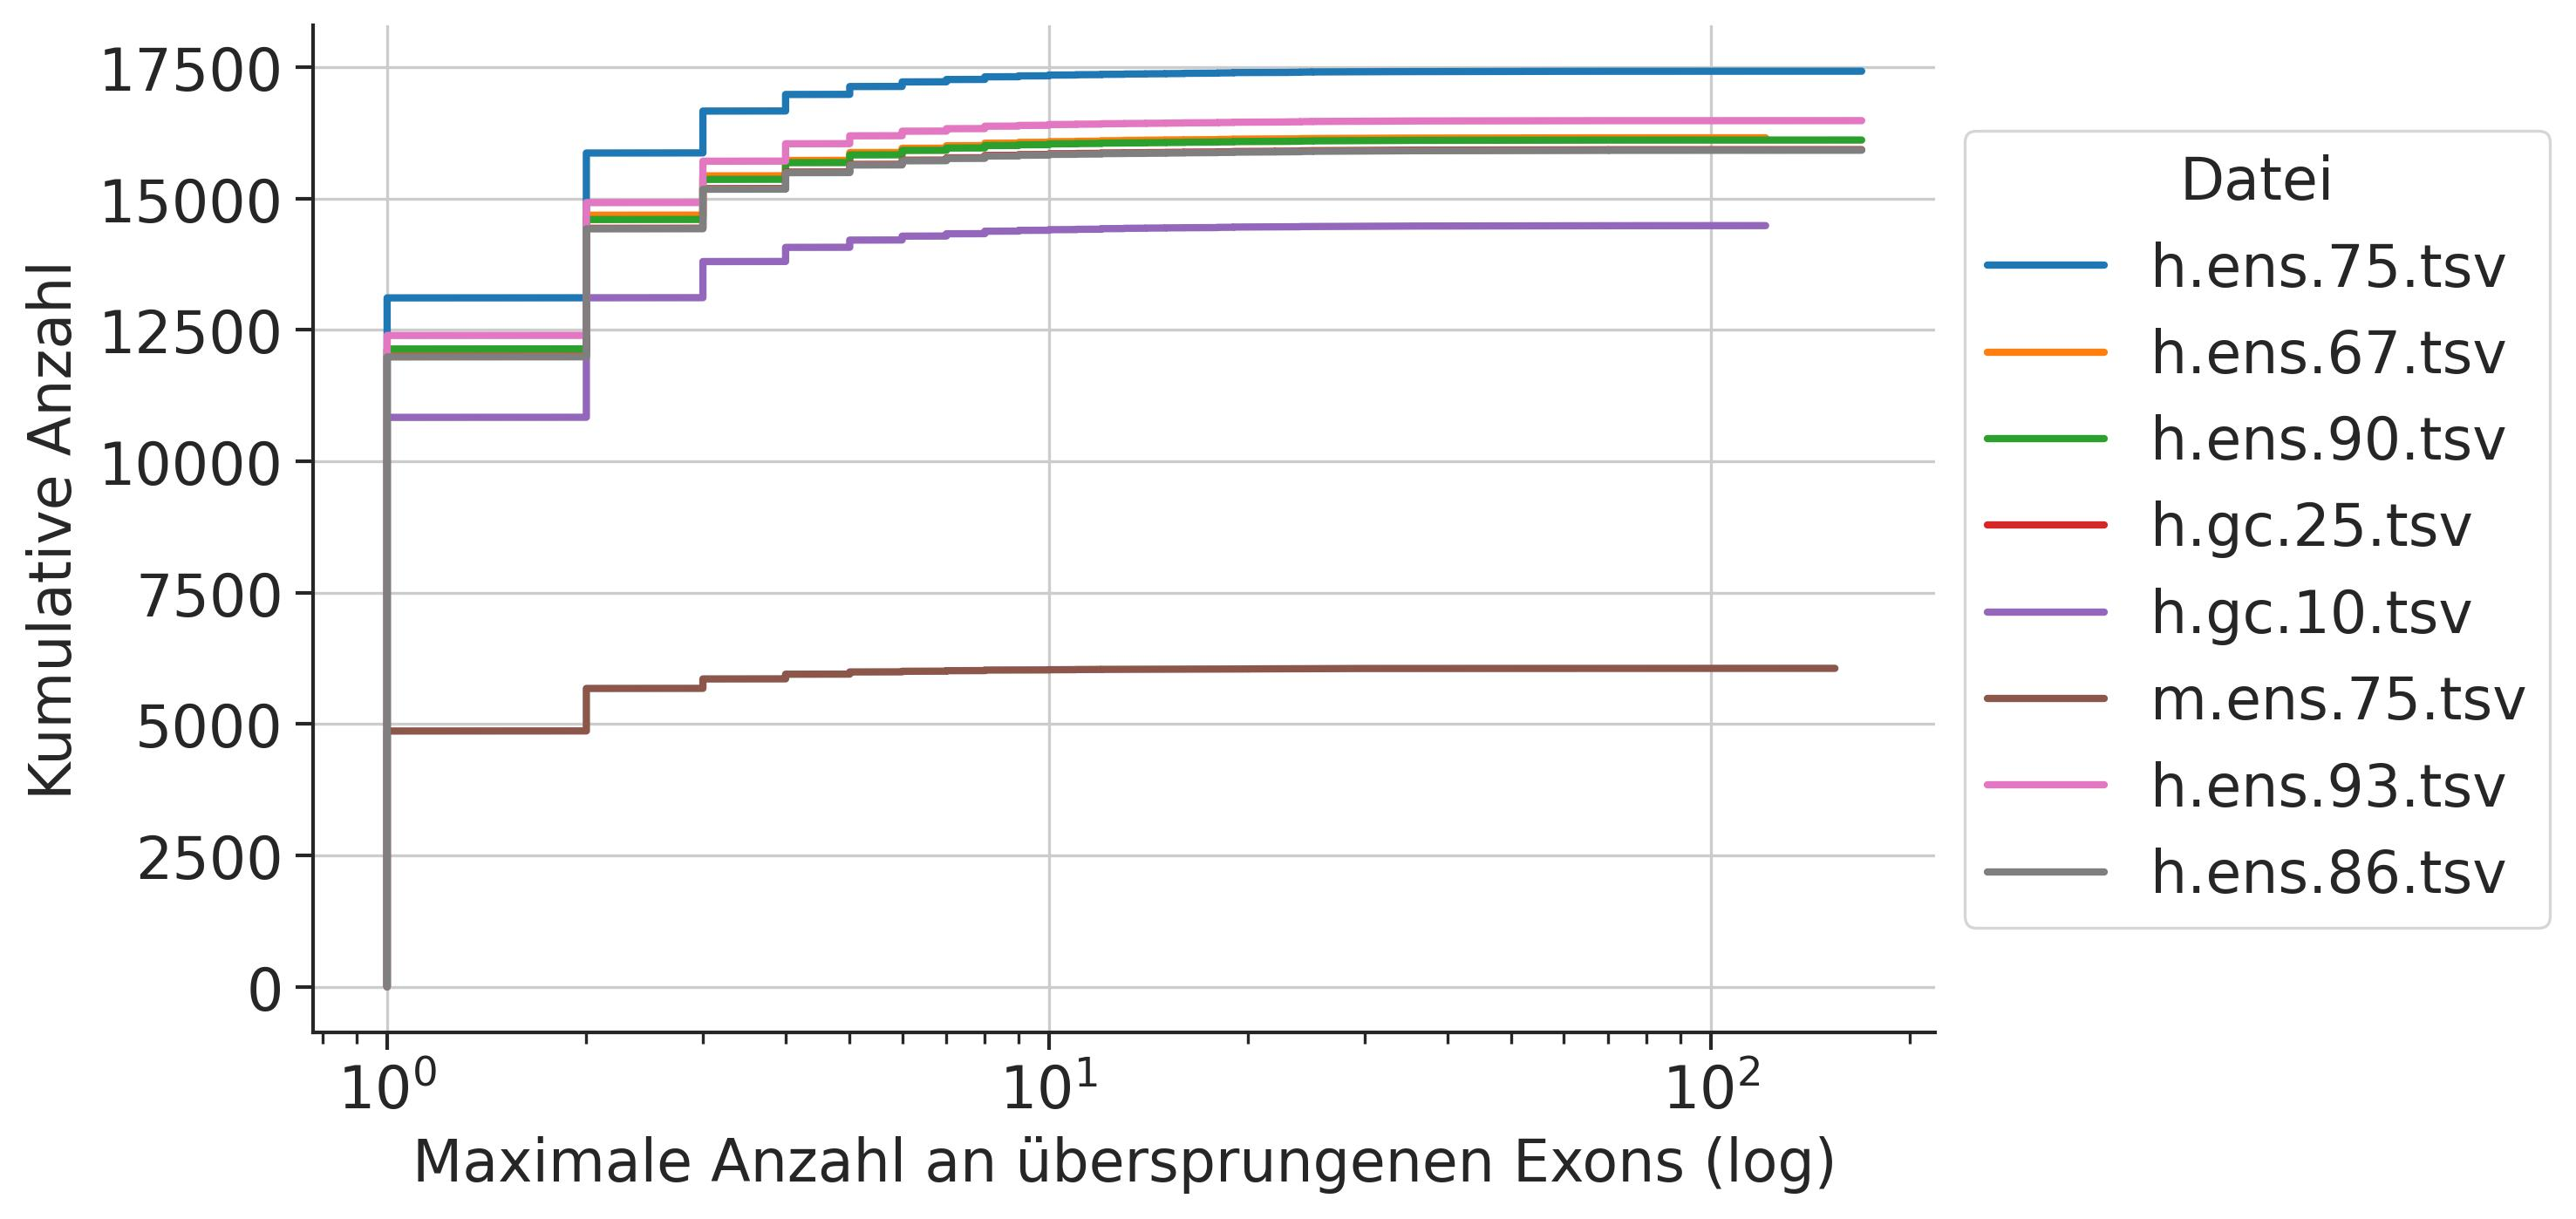
\includegraphics[width=0.8\textwidth]{./plots/skipped_exons.jpg}
	\caption{Kumulative Verteilung der übersprungenen Exons pro \textit{GTF}}
	\label{fig:-plots-skipped_exons-jpg}
\end{figure}

Abbildung \ref{fig:-plots-skipped_exons-jpg} zeigt die kumulative Verteilung der übersprungenen Exons pro \textit{GTF}.
Auch hier zeigen sich die 4 Trends aus \ref{fig:-plots-skipped_bases-jpg} und \ref{fig:-plots-genes-jpg}.
Die meisten \textit{ES-SE} betreffen lediglich ein oder zwei Exons und werden mit zunehmender Anzahl an
übersprungenen Exons immer weniger.
Diese Verteilung unterstreicht die biologische Relevanz von \textit{Single-Exon-Skipping} als häufigstem Mechanismus im alternativen
Spleißen und zeigt gleichzeitig, dass komplexere \textit{ES-SE} mit mehreren Exons zwar vorkommen,
aber deutlich seltener sind.







\begin{figure}[htbp]
	\centering
	% First table in a minipage
	\begin{minipage}{0.45\textwidth}
		\centering
		\caption{Übersprungene Basen}
		\begin{tabular}{l|l}
			\textit{\textbf{gene\_id}}                 & \textit{\textbf{skipped\_bases}} \\\hline
            \href{https://asia.ensembl.org/Homo_sapiens/Gene/Summary?db=core;g=ENSG00000155657;r=2:178525989-178830802}{ENSG00000155657}    & 26106               \\
            \href{https://asia.ensembl.org/Homo_sapiens/Gene/Summary?db=core;g=ENSG00000155657;r=2:178525989-178830802}{ENSG00000155657.25} & 26106               \\
            \href{https://asia.ensembl.org/Mus_musculus/Gene/Summary?db=core;g=ENSMUSG00000051747;r=2:76534324-76812891}{\textbf{ENSMUSG00000051747}} & 24843               \\
            \href{https://asia.ensembl.org/Homo_sapiens/Gene/Idhistory?g=ENSG00000283186}{ENSG00000283186}    & 22134               \\
            \href{https://asia.ensembl.org/Homo_sapiens/Gene/Summary?db=core;g=ENSG00000155657;r=2:178525989-178830802}{ENSG00000155657.16} & 22134               \\
            \href{https://asia.ensembl.org/Homo_sapiens/Gene/Idhistory?g=ENSG00000283186}{ENSG00000283186.1}  & 22134               \\
            \href{https://asia.ensembl.org/Homo_sapiens/Gene/Summary?db=core;g=ENSG00000145113;r=3:195746765-195811973}{ENSG00000145113}    & 12875               \\
            \href{https://asia.ensembl.org/Homo_sapiens/Gene/Summary?db=core;g=ENSG00000145113;r=3:195746765-195811973}{ENSG00000145113.16} & 12875               \\
            \href{https://asia.ensembl.org/Homo_sapiens/Gene/Summary?db=core;g=ENSG00000145113;r=3:195746765-195811973}{ENSG00000145113.21} & 12875               \\
            \href{https://asia.ensembl.org/Homo_sapiens/Gene/Summary?db=core;g=ENSG00000164199;r=5:90529344-91164437}{ENSG00000164199}    & 12530               \\
		\end{tabular}
	\end{minipage}%
	\hfill % Adds horizontal space between the tables
	% Second table in a minipage
	\begin{minipage}{0.45\textwidth}
		\centering
		\caption{Übersprungene Exons}
		\begin{tabular}{l|l}
			\textit{\textbf{gene\_id}}                 & \textit{\textbf{skipped\_exons}} \\\hline
            \href{https://asia.ensembl.org/Homo_sapiens/Gene/Summary?db=core;g=ENSG00000155657;r=2:178525989-178830802}{ENSG00000155657}    & 169                \\
            \href{https://asia.ensembl.org/Homo_sapiens/Gene/Summary?db=core;g=ENSG00000155657;r=2:178525989-178830802}{ENSG00000155657.25} & 169                \\
            \href{https://asia.ensembl.org/Mus_musculus/Gene/Summary?db=core;g=ENSMUSG00000051747;r=2:76534324-76812891}{\textbf{ENSMUSG00000051747}} & 154                \\
            \href{https://asia.ensembl.org/Homo_sapiens/Gene/Idhistory?g=ENSG00000283186}{ENSG00000283186}    & 121                \\
            \href{https://asia.ensembl.org/Homo_sapiens/Gene/Summary?db=core;g=ENSG00000155657;r=2:178525989-178830802}{ENSG00000155657.16} & 121                \\
            \href{https://asia.ensembl.org/Homo_sapiens/Gene/Idhistory?g=ENSG00000283186}{ENSG00000283186.1}  & 121                \\
            \href{https://asia.ensembl.org/Homo_sapiens/Gene/Idhistory?g=ENSG00000203832}{ENSG00000203832.5}  & 78                 \\
            \href{https://asia.ensembl.org/Homo_sapiens/Gene/Summary?db=core;g=ENSG00000187240;r=11:103109410-103479863}{ENSG00000187240}    & 70                 \\
            \href{https://asia.ensembl.org/Homo_sapiens/Gene/Summary?db=core;g=ENSG00000271425;r=1:146064711-146229000}{ENSG00000271425}    & 70                 \\
            \href{https://asia.ensembl.org/Homo_sapiens/Gene/Summary?db=core;g=ENSG00000187240;r=11:103109410-103479863}{ENSG00000187240.8}  & 70                 \\
		\end{tabular}
	\end{minipage}
\end{figure}



% ------------------------------------------------------------------------------








% ------------------------------------------------------------------------------
% \printbibliography
% ------------------------------------------------------------------------------


% ------------------------------------------------------------------------------
\newpage~\appendix
% ------------------------------------------------------------------------------

\section{Appendix Section}

hm

Text goes here



\end{document}
